\usepackage{xcolor}
\usepackage{titleps}
\usepackage[letterpaper, margin=0.95in]{geometry}
\usepackage{url}
\usepackage{amsmath}
\usepackage{amsfonts}
\usepackage{amssymb}
\usepackage{wrapfig}
\usepackage{float}
\usepackage{mathtools}
\usepackage{enumitem}
\usepackage{tabu}
\usepackage{parskip}
\usepackage{natbib}
\usepackage{listings}
\usepackage{tcolorbox}
\usepackage{algorithm}
\usepackage{algpseudocode}
\usepackage{forest}
\usepackage{hyperref}
\usepackage[color=red]{todonotes}
\usepackage{forest}
\definecolor{light-yellow}{HTML}{FFE5CC}
\usepackage{cleveref}

\newcommand{\xb}{\mathbf{x}}
\newcommand{\yb}{\mathbf{y}}
\newcommand{\wb}{\mathbf{w}}
\newcommand{\Xb}{\mathbf{X}}
\newcommand{\Yb}{\mathbf{Y}}
\newcommand{\tr}{^T}
\newcommand{\hb}{\mathbf{h}}
\newcommand{\Hb}{\mathbf{H}}

\DeclareFontShape{OT1}{cmtt}{bx}{n}{<5><6><7><8><9><10><10.95><12><14.4><17.28><20.74><24.88>cmttb10}{}

\newpagestyle{ruled}
{\sethead{Berkeley CS 285}{Deep Reinforcement Learning, Decision Making, and Control}{Fall 2022}\headrule
  \setfoot{}{\ifsolutions\LARGE\bf\textcolor{red}{Answer Key}\fi}{}}
\pagestyle{ruled}

\renewcommand\makeheadrule{\color{black}\rule[-.75\baselineskip]{\linewidth}{0.4pt}}
\renewcommand*\footnoterule{}

\newcommand*{\MYSOLUTION}[0]{\textcolor{red}{\textbf{My Solution: }}}

\begin{document}
\lstset{basicstyle = \ttfamily,columns=fullflexible,
backgroundcolor = \color{light-yellow}
}

\begin{centering}
    {\Large Assignment 3: Q-Learning and Actor-Critic Algorithms} \\
    \vspace{.25cm}
    \textbf{Due October 18, 11:59 pm} \\
\end{centering}

\section{Multistep Q-Learning}

\ifsolutions
\input{hw3_solutions/01_solutions}
\fi

\def\solve#1{\csname solution to #1\endcsname}

\begingroup
\def\Q{Q_{\phi_k}}
\def\Qn{Q_{\phi_{k+1}}}
\def\D{\mathcal{D}}

Consider the $N$-step variant of Q-learning described in lecture. We learn $\Qn$ with the following updates:\begin{align}
  y_{j,t} &\gets \biggl(\;\sum_{t'=t}^{t+N-1} \gamma^{t'-t} r_{j,t'}\biggr)+\gamma^{N} \max _{\mathbf{a}_{j,t+N}} \Q\left(\mathbf{s}_{j,t+N}, \mathbf{a}_{j,t+N}\right) \label{eq:q_target}\\
  \phi_{k+1} &\gets \underset{\phi\in\Phi}{\arg\min}  \sum_{j,t} \bigl( y_{j,t}-Q_{\phi}(\mathbf s_{j,t},\mathbf a_{j,t}) \bigr)^2 \label{eq:q_update}
\end{align}
In these equations, $j$ indicates an index in the replay buffer of trajectories $\D_k$. We first roll out a batch of $B$ trajectories to update $\D_k$ and compute the target values in \eqref{eq:q_target}. We then fit $\Qn$ to these target values with \eqref{eq:q_update}. 
After estimating $\Qn$, we can then update the policy through an argmax:\begin{align}
  \pi_{k+1}\left(\mathbf{a}_{t} \mid \mathbf{s}_{t}\right)\gets \left\{\begin{array}{l}1 \text { if } \mathbf{a}_{t}=\arg \max _{\mathbf{a}_{t}} Q_{\phi_{k+1}}\left(\mathbf{s}_{t}, \mathbf{a}_{t}\right) \\ 0 \text{ otherwise. }\end{array}\right. \label{eq:policy_improvement}
\end{align}
We repeat the steps in \cref{eq:q_target,eq:q_update,eq:policy_improvement} $K$ times to improve the policy. In this question, you will analyze some properties of this algorithm, which is summarized in \Cref{alg:multi}.

\begin{algorithm}
\caption{Multistep Q-Learning}
\label{alg:multi}
\begin{algorithmic}[1]
	\Require{iterations $K$, batch size $B$}
	\State initialize random policy $\pi_0$, sample $\phi_0\sim\Phi$
	\For{$k=0\ldots K-1$}
		\State Update $\D_{k+1}$ with $B$ new rollouts from $\pi_k$ \label{eq:data}
		\State compute targets with \eqref{eq:q_target}
		\State $Q_{\phi_{k+1}} \gets$ update with \eqref{eq:q_update}
		\State $\pi_{k+1} \gets$ update with \eqref{eq:policy_improvement}
	\EndFor
	\State\Return $\pi_{K}$
\end{algorithmic}	
\end{algorithm}



\def\makecols#1#2{{\def\p{#2}\newcount\i\i0\hfill\loop\advance\i1\makebox[1cm][c]{\expandafter\p\the\i}\kern.5cm\ifnum\i<#1\repeat\kern-1cm}}
\def\heading#1{\bf\expandafter\uppercase\expandafter{\romannumeral#1.}}
\def\boxes#1{\ensuremath\square}
\def\filled#1#2|#3{\ifnum#1=#3\ensuremath\blacksquare
	\else\if\relax#2\relax\ensuremath\square
	\else\filled#2|#3\fi\fi}
\def\ncol{3}
\newcommand{\checkeditem}[2]{\edef\x{0#1}\item[\expandafter\filled\x|#2]}


\def\choices#1#2{
	\begin{enumerate}
	\item on-policy in tabular setting \makecols\ncol{\filled0#1|}
	\item off-policy in tabular setting \makecols\ncol{\filled0#2|}
	\end{enumerate}
}

\subsection{TD-Learning Bias (2 points)}
\label{q:td_bias}

\def\answer{} % <--- TODO: insert index (0/1) of answer
\ifsolutions\solve\thesubsection\fi
We say an estimator $f_\D$ of $f$ constructed using data $\D$ sampled from process $P$ is \textit{unbiased} when $\mathbb{E}_{\D\sim P}[f_\D(x)-f(x)]=0$ at each $x$.

Assume $\hat Q$ is a noisy (but unbiased) estimate for $Q$. Is the Bellman backup $\mathcal{B}\hat Q = r(s, a) + \gamma \max_{a'} \hat Q(s', a')$ an unbiased estimate of $\mathcal{B}Q$?
\begin{itemize}
    \checkeditem\answer1 Yes
    \checkeditem\answer2 No
\end{itemize}

\subsection{Tabular Learning (6 points total)}
\label{q:tabular_learning}

At each iteration of the algorithm above after the update from \cref{eq:q_update}, $\Q$ can be viewed as an estimate of the true optimal $Q^*$. Consider the following statements: 
\begin{enumerate}[label=\bf\Roman*.]
  \item $Q_{\phi_{k+1}}$ is an unbiased estimate of the $Q$ function of the last policy, $Q^{\pi_k}$.
  \item As $k\to\infty$ for some fixed $B$, $\Q$ is an unbiased estimate of $Q^*$, i.e., $\lim_{k\to\infty} \mathbb{E}\bigl[\Q(s,a)-Q^*(s,a)]=0$.
  \item In the limit of infinite iterations and data we recover the optimal $Q^*$, i.e., $\lim_{k,B\to\infty}\mathbb{E}\,\bigl[\|\Q-Q^*\|_\infty\bigr]=0$.
\end{enumerate}

We make the additional assumptions: 
\begin{itemize}
	\item The state and action spaces are finite.
	\item Every batch contains at least one experience for each action taken in each state.
	\item In the tabular setting, $\Q$ can express any function, i.e., $\{\Q:\phi\in\Phi\}=\mathbb{R}^{S\times A}$.
\end{itemize}
When updating the buffer $\D_k$ with $B$ new trajectories in \cref{eq:data} of \Cref{alg:multi}, we say:
\begin{itemize}
    \item When learning \textit{on-policy}, $\D_k$ is set to contain only the set of $B$ new rollouts of $\pi$ (so $\lvert \D_k \rvert = B$). Thus, we only train on rollouts from the current policy.
	\item When learning \textit{off-policy}, we use a fixed dataset $\D_k=\D$ of $B$ trajectories from another policy $\pi'$. 
\end{itemize}

Indicate which of the statements \textbf{I-III} always hold in the following cases. No justification is required.
\ifsolutions\solve\thesubsection\else
\begin{enumerate}
\item $N=1$ and \ldots \makecols\ncol\heading\choices
	{} % <--- TODO: select numbers of boxes to fill; e.g., {13} to select I and III
	{} % <--- TODO: "
\item $N>1$ and \ldots \choices
	{} % <--- TODO: "
	{} % <--- TODO: "
\item In the limit as $N\to\infty$ (no bootstrapping) \ldots \choices
	{} % <--- TODO: "
	{} % <--- TODO: "
\end{enumerate}
\fi

\subsection{Variance of $Q$ Estimate (2 points)}
\label{q:variance_estimate}
Which of the three cases ($N = 1$, $N > 1$, $N \to \infty$) would you expect to have the highest-variance estimate of $Q$ for fixed dataset size $B$ in the limit of infinite iterations $k$? Lowest-variance?

\def\highest{} % <--- TODO: insert index of highest variance answer
\def\lowest{} % <--- TODO: insert index of lowest variance answer
\ifsolutions\solve\thesubsection\fi
\begin{minipage}{0.49\linewidth}
Highest variance:\smallskip
\begin{itemize}\itemsep=1ex
    \checkeditem\highest1 $N = 1$
    \checkeditem\highest2 $N > 1$
    \checkeditem\highest3 $N \to \infty$
\end{itemize}
\end{minipage}
\begin{minipage}{0.49\linewidth}
Lowest variance:\smallskip
\begin{itemize}\itemsep=1ex
    \checkeditem\lowest1 $N = 1$
    \checkeditem\lowest2 $N > 1$
    \checkeditem\lowest3 $N \to \infty$
\end{itemize}
\end{minipage}

\subsection{Function Approximation (2 points)}
\label{q:function_approximation}
Now say we want to represent $Q$ via function approximation rather than with a tabular representation. Assume that for any deterministic policy $\pi$ (including the optimal policy $\pi^*$), function approximation can represent the true $Q^\pi$ exactly.
Which of the following statements are true?

\def\answer{} % <--- TODO: insert index of answer(s)
\ifsolutions\solve\thesubsection\fi
\begin{itemize}
    \checkeditem\answer1 When $N = 1$, $Q_{\phi_{k+1}}$ is an unbiased estimate of the $Q$-function of the last policy $Q^{\pi_k}$.
    \checkeditem\answer2 When $N = 1$ and in the limit as $B\to\infty,\,k \to \infty$, $\Q$ converges to $Q^*$.
    \checkeditem\answer3 When $N > 1$ (but finite) and in the limit as $B\to\infty,\,k \to \infty$, $\Q$ converges to $Q^*$.
    \checkeditem\answer4 When $N \to \infty$ and in the limit as $B \to \infty,\,k \to \infty$, $\Q$ converges to $Q^*$.
\end{itemize}

\subsection{Multistep Importance Sampling (5 points)}
\label{q:importance_sampling}

We can use importance sampling to make the $N$-step update work off-policy with trajectories drawn from an arbitrary policy. Rewrite \eqref{eq:q_update} to correctly approximate a $\Q$ that improves upon $\pi$ when it is trained on data $\D$ consisting of $B$ rollouts of some other policy $\pi'(\mathbf a_t\mid\mathbf s_t)$. 

Do we need to change \eqref{eq:q_update} when $N=1$? What about as $N\to\infty$? 

You may assume that $\pi'$ always assigns positive mass to each action. [Hint: re-weight each term in the sum using a ratio of likelihoods from the policies $\pi$ and $\pi'$.]

 
\ifsolutions\solve\thesubsection\else
% TODO: answer question above
\fi

\endgroup

\section{Deep Q-Learning}
\subsection{Introduction}

Part 1 of this assignment requires you to implement and evaluate Q-learning for playing Atari games. The Q-learning algorithm was covered in lecture, and you will be provided with starter code. This assignment will be faster to run on a GPU, though it is possible to complete on a CPU as well. Note that we use convolutional neural network architectures in this assignment. Therefore, we recommend using the Colab option if you do not have a GPU available to you. Please start early!

% The questions will require you to perform multiple runs of Q-learning, each of which can take quite a long time. Furthermore, depending on your implementation, you may find it necessary to tweak some of the parameters, such as learning rates or exploration schedules, which can also be very time consuming. The actual coding for this assignment will involve about 50 lines of code, but the evaluation will take longer than in the previous two assignments.

\subsection{File overview}
The starter code for this assignment can be found at

\begin{centering}
\url{https://github.com/berkeleydeeprlcourse/homework_fall2023/tree/main/hw3} \\
\end{centering}
\vspace{.35cm}

You will implement a DQN agent in \verb|cs285/agents/dqn_agent.py| and \verb|cs285/scripts/run_hw3_dqn.py|. In addition to those two files, you should start by reading the following files thoroughly:
\begin{itemize}
    \item \verb|cs285/env_configs/dqn_basic.py|: builds networks and generates configuration for the basic DQN problems (cartpole, lunar lander).
    \item \verb|cs285/env_configs/dqn_atari.py|: builds networks and generates configuration for the Atari DQN problems.
    \item \verb|cs285/infrastructure/replay_buffer.py|: implementation of replay buffer. You don't need to know how the memory efficient replay buffer works, but you should try to understand what each method does (particularly the difference between \verb|insert|, which is called after a frame, and \verb|on_reset|, which inserts the first observation from a trajectory) and how it differs from the regular replay buffer.
    \item \verb|cs285/infrastructure/atari_wrappers.py|: contains some wrappers specific to the Atari environments. These wrappers can be key to getting challenging Atari environments to work!
\end{itemize}

There are two new package requirements (\texttt{gym[atari]} and \texttt{pip install gym[accept-rom-license]}) beyond what was used in the first two assignments; make sure to install these with \texttt{pip install -r requirements.txt} if you're re-using your Python environment from last assignment.

\subsection{Implementation}

The first phase of the assignment is to implement a working version of Q-learning, with some extra bells and whistles like double DQN. Our code will work with both state-based environments, where our input is a low-dimensional list of numbers (like Cartpole), but we'll also support learning directly from pixels!

In addition to the double $Q$-learning trick (which you'll implement later), we have a few other tricks implemented to stabilize performance. You don't have to do anything to enable these, but you should look at the implementations and think about why they work.
\begin{itemize}
    \item \textbf{Exploration scheduling for $\epsilon$-greedy actor.} This starts $\epsilon$ at a high value, close to random sampling, and decays it to a small value during training.
    \item \textbf{Learning rate scsheduling.} Decay the learning rate from a high initial value to a lower value at the end of training.
    \item \textbf{Gradient clipping.} If the gradient norm is larger than a threshold, scale the gradients down so that the norm is equal to the threshold.
    \item \textbf{Atari wrappers.}
    \begin{itemize}
        \item \textbf{Frame-skip.} Keep the same constant action for 4 steps.
        \item \textbf{Frame-stack.} Stack the last 4 frames to use as the input.
        \item \textbf{Grayscale.} Use grayscale images.
        % \item \textbf{Fire-reset.} Some Atari games require pressing the ``fire'' button to start the game. In these environments, do this automatically.
    \end{itemize}
\end{itemize}

\subsection{Basic Q-Learning}

Implement the basic DQN algorithm. You'll implement an update for the $Q$-network, a target network, and 

\textbf{What you'll need to do}:
\begin{itemize}
    \item Implement a DQN critic update in \verb|update_critic| by filling in the unimplemented sections (marked with TODO(student)).
    \item Implement $\epsilon$-greedy sampling in \verb|get_action|
    \item Implement the TODOs in \verb|run_hw3_dqn.py|.

    \textbf{Hint:} A trajectory can end (\verb|done=True|) in two ways: the actual end of the trajectory (usually triggered by catastrophic failure, like crashing), or \textit{truncation}, where the trajectory doesn't actually end but we stop simulation for some reason (commonly, we truncate trajectories at some maximum episode length). In this latter case, you should still reset the environment, but the \verb|done| flag for TD-updates (stored in the replay buffer) should be false.
    \item Call all of the required updates, and update the target critic if necessary, in \verb|update|.
\end{itemize}

\textbf{Testing this section}:
\begin{itemize}
    \item Debug your DQN implementation on \verb|CartPole-v1| with \verb|experiments/dqn/cartpole.yaml|. It should reach reward of nearly 500 within a few thousand steps.
\end{itemize}

\textbf{Deliverables}:
\begin{itemize}
    \item Submit your logs of \verb|CartPole-v1|, and a plot with environment steps on the $x$-axis and eval return on the $y$-axis.
    
\MYSOLUTION



    \item Run DQN with three different seeds on \verb|LunarLander-v2|:
\begin{lstlisting}[language=bash,breaklines=true]
  python cs285/scripts/run_hw3_dqn.py -cfg experiments/dqn/lunarlander.yaml --seed 1
  python cs285/scripts/run_hw3_dqn.py -cfg experiments/dqn/lunarlander.yaml --seed 2
  python cs285/scripts/run_hw3_dqn.py -cfg experiments/dqn/lunarlander.yaml --seed 3
\end{lstlisting}
\textbf{Your code may not reach high return (200) on Lunar Lander yet; this is okay!} Your returns may go up for a while and then collapse in some or all of the seeds.
    \item Run DQN on \verb|CartPole-v1|, but change the \verb|learning rate| to 0.05 (you can change this in the YAML config file). What happens to (a) the predicted $Q$-values, and (b) the critic error? Can you relate this to any topics from class or the analysis section of this homework?
\end{itemize}

\subsection{Double Q-Learning}
Let's try to stabilize learning. The double-Q trick avoids overestimation bias in the critic update by using two different networks to \textit{select} the next action $a'$ and to \textit{estimate} its value:
\[a' = \textrm{arg}\max_{a'} Q_{\phi}(s', a')\]
\[Q_{\textrm{target}} = r + \gamma(1-d_t) Q_{\phi'}(s', a').\]
In our case, we'll keep using the target network $Q_{\phi'}$ to estimate the action's value, but we'll select the action using $Q_{\phi}$ (the online $Q$ network).

Implement this functionality in \verb|dqn_agent.py|.

\textbf{Deliverables}:
\begin{itemize}
    \item Run three more seeds of the lunar lander problem:
\begin{lstlisting}[language=bash,breaklines=true]
  python cs285/scripts/run_hw3_dqn.py -cfg experiments/dqn/lunarlander_doubleq.yaml --seed 1
  python cs285/scripts/run_hw3_dqn.py -cfg experiments/dqn/lunarlander_doubleq.yaml --seed 2
  python cs285/scripts/run_hw3_dqn.py -cfg experiments/dqn/lunarlander_doubleq.yaml --seed 3
\end{lstlisting}
    You should expect a return of \textbf{200} by the end of training, and it should be fairly stable compared to your policy gradient methods from HW2.
    
    Plot returns from these three seeds in red, and the ``vanilla'' DQN results in blue, on the same set of axes. Compare the two, and describe in your own words what might cause this difference.

    \item Run your DQN implementation on the \verb|MsPacman-v0| problem. Our default configuration will use double-$Q$ learning by default. You are welcome to tune hyperparameters to get it to work better, but the default parameters should work (so if they don't, you likely have a bug in your implementation). Your implementation should receive a score of around \textbf{1500} by the end of training (1 million steps. \textbf{This problem will take about 3 hours with a GPU, or {\color{red} 6 hours} without, so start early!}
    \begin{lstlisting}[language=bash,breaklines=true]
    python cs285/scripts/run_hw3_dqn.py -cfg experiments/dqn/mspacman.yaml
    \end{lstlisting}
    \item Plot the average training return (\verb|train_return|) and eval return (\verb|eval_return|) on the same axes. You may notice that they look very different early in training! Explain the difference.
\end{itemize}

\subsection{Experimenting with Hyperparameters} Now let's analyze the sensitivity of Q-learning to hyperparameters. Choose one hyperparameter of your choice and run at least three other settings of this hyperparameter, in addition to the one used in Question 1, and plot all four values on the same graph. Your choice what you experiment with, but you should explain why you chose this hyperparameter in the caption. Create four config files in \verb|experiments/dqn/hyperparameters|, and look in \verb|cs285/env_configs/basic_dqn_config.py| to see which hyperparameters you're able to change. You can use any of the base YAML files as a reference.

Hyperparameter options could include:
\begin{itemize}
    \item Learning rate
    \item Network architecture
    \item Exploration schedule (or, if you'd like, you can implement an alternative to $\epsilon$-greedy)
\end{itemize}
\section{Continuous Actions with Actor-Critic}
DQN is great for discrete action spaces. However, it requires you to be able to calculate $\max_a Q(s, a)$ in closed form. Doing this is trivial for discrete action spaces (when you can just check which of the $n$ actions has the highest $Q$-value), but in continuous action spaces this is potentially a complex nonlinear optimization problem.

Actor-critic methods get around this by learning two networks: a $Q$-function, like DQN, and an explicit policy $\pi$ that is trained to maximize $\mathbb{E}_{a \sim \pi(a|s)} Q(s, a)$.

All parts in this section are run with the following command:
\begin{lstlisting}[language=bash,breaklines=true]
  python cs285/scripts/run_hw3_sac.py -cfg experiments/sac/<CONFIG>.yaml
\end{lstlisting}

\subsection{Implementation}
First, you'll need to take a look at the following files:
\begin{itemize}
    \item \verb|cs285/scripts/run_hw3_sac.py| - the main training loop for your SAC implementation.
    \item \verb|cs285/agents/soft_actor_critic.py| - the structure for the SAC learner you'll implement.
\end{itemize}
You may also find the following files useful:
\begin{itemize}
    \item \verb|cs285/networks/state_action_critic.py| - a simple MLP-based $Q(s, a)$ network. Note that unlike the DQN critic, which maps states to an array of $Q$-value, one per action, this critic maps one $(s, a)$ pair to a single $Q$-value.
    \item \verb|cs285/env_configs/sac_config.py| - base configuration (and list of hyperparameters).
    \item \verb|experiments/sac/*.yaml| - configuration files for the experiments.
\end{itemize}

You'll primarily be implementing your code in \verb|cs285/agents/soft_actor_critic.py|.

\textbf{Before implementing SAC:}
\begin{itemize}
    \item Fill in all of the \verb|TODO|s in \verb|cs285/scripts/run_hw3_sac.py|. This should look pretty similar to your DQN run script, as both are off-policy methods!
\end{itemize}

\subsubsection{Bootstrapping}
As in DQN, we train our critic by ``bootstrapping'' from a target critic. Using the tuple $(s_t, a_t, r_t, s_{t+1}, d_{t})$ (where $d_t$ is the flag for whether the trajectory terminates after this transition), we write:
\[y \gets r_t + \gamma (1-d_t) Q_\phi(s_{t+1}, a_{t+1}), a \sim \pi(a_{t+1}|s_{t+1})\]
\[\min_\phi (Q_\phi(s_t, a_t) - y)^2\]
In practice, we stabilize learning by using a separate \textit{target network} $Q_{\phi'}$. There are two common strategies for updating the target network:
\begin{itemize}
    \item \textit{Hard update} (like we implemented in DQN), where every $K$ steps we set $\phi' \gets \phi$.
    \item \textit{Soft update}, where $\phi'$ is continually updated towards $\phi$ with \textit{Polyak averaging} (exponential moving average). After each step, we perform the following operation:
    \[\phi' \gets \phi' + \tau(\phi-\phi')\]
\end{itemize}

\textbf{What you'll need to do} (in \verb|cs285/agents/soft_actor_critic.py|):
\begin{itemize}
    \item Implement the bootstrapped critic update in the \verb|update_critic| method.
    \item Update the critic for \verb|num_critic_updates| in the \verb|update| method.
    \item Implement soft and hard target network updates, depending on the configuration, in \verb|update|.
\end{itemize}

\textbf{Testing this section}:
\begin{itemize}
    \item Train an agent on \verb|Pendulum-v1| with the sample configuration \verb|experiments/sac/sanity_pendulum.yaml|. It shouldn't get high reward yet (you're not training an actor), but the $Q$-values should stabilize at some large negative number. The ``do-nothing'' reward for this environment is about -10 per step; you can use that together with the discount factor $\gamma$ to calculate (approximately) what $Q$ should be. If the $Q$-values go to minus infinity or stay close to zero, you probably have a bug.
\end{itemize}

\textbf{Deliverables}: None, once the critic is training as expected you can move on to the next section!

\subsubsection{Entropy Bonus and Soft Actor-Critic}
In DQN, we used an $\epsilon$-greedy strategy to decide which action to take at a given time. In continuous spaces, we have several options for generating exploration noise.

One of the most common is providing an \textit{entropy bonus} to encourage the actor to have high entropy (i.e. to be ``more random''), scaled by a ``temperature'' coefficient $\beta$. For example, in the REPARAMETRIZE case:
\[\mathcal L_\pi = Q(s, \mu_\theta(s) + \sigma_\theta(s)\epsilon) + \beta\mathcal{H}(\pi(a|s)).\]
Where entropy is defined as $\mathcal H(\pi(a|s)) = \mathbb{E}_{a \sim \pi}\left[-\log\pi(a|s)\right]$. To make sure entropy is also factored into the $Q$-function, we should also account for it in our target values:
\[y \gets r_t + \gamma(1-d_t)\left[Q_\phi(s_{t+1}, a_{t+1}) + \beta\mathcal{H}(\pi(a_{t+1}|s_{t+1}))\right]\]
When balanced against the ``maximize $Q$'' terms, this results in behavior where the actor will choose more random actions when it is unsure of what action to take.
Feel free to read more in the SAC paper: {\url{https://arxiv.org/abs/1801.01290 }}.

Note that maximizing entropy $\mathcal{H}(\pi_\theta) = -\mathbb{E}[\log \pi_\theta]$ requires differentiating \textit{through} the sampling distribution. We can do this via the ``reparametrization trick'' from lecture - if you'd like a refresher, skip to the section on REPARAMETRIZE.

\textbf{What you'll need to do} (in \verb|cs285/agents/soft_actor_critic.py|):
\begin{itemize}
    \item Implement \verb|entropy()| to calculate the approximate entropy of an actor distribution.
    \item Add the entropy term to the target critic values in \verb|update_critic()| and the actor loss in \verb|update_actor()|.
\end{itemize}

\textbf{Testing this section}:
\begin{itemize}
    \item The code should be logging \verb|entropy| during the critic updates. If you run \verb|sanity_pendulum.yaml| from before, it should achieve (close to) the maximum possible entropy for a 1-dimensional action space. Entropy is maximized by a uniform distribution:
    \[\mathcal{H}(\mathcal{U}[-1, 1]) = \mathbb{E}[-\log p(x)] = -\log \frac{1}{2} = \log 2 \approx 0.69\]
    Because currently our actor loss \textbf{only} consists of the entropy bonus (we haven't implemented anything to maximize rewards yet), the entropy should increase until it arrives at roughly this level.

    If your logged entropy is higher than this, or significantly lower, you have a bug.
\end{itemize}

\subsubsection{Actor with REINFORCE}
We can use the same REINFORCE gradient estimator that we used in our policy gradients algorithms to update our actor in actor-critic algorithms! We want to compute:
\[\nabla_\theta\mathbb{E}_{s \sim \mathcal{D}, a \sim \pi_\theta(a|s)}\left[Q(s, a)\right]\]
To do this using REINFORCE, we can use the policy gradient:
\[\mathbb{E}_{s \sim \mathcal{D}, a \sim \pi(a|s)}\left[\nabla_\theta \log(\pi_\theta(a|s))Q_\phi(s, a)\right]\]
Note that the actions $a$ are sampled from $\pi_\theta$, and we do \textbf{not} require real data samples. This means that to reduce variance we can just sample more actions from $\pi$ for any given state! You'll implement this in your code using the \verb|num_actor_samples| parameter.

\textbf{What you'll need to do} (in \verb|cs285/agents/soft_actor_critic.py|):
\begin{itemize}
    \item Implement the REINFORCE gradient estimator in the \verb|actor_loss_reinforce| method.
    \item Update the actor in \verb|update|.
\end{itemize}

\textbf{Testing this section}:
\begin{itemize}
    \item Train an agent on \verb|InvertedPendulum-v4| using \verb|sanity_invertedpendulum_reinforce.yaml|. You should achieve reward close to 1000, which corresponds to staying upright for all time steps.
\end{itemize}

\MYSOLUTION The result is shown below.

\begin{figure}[H]
    \centering
    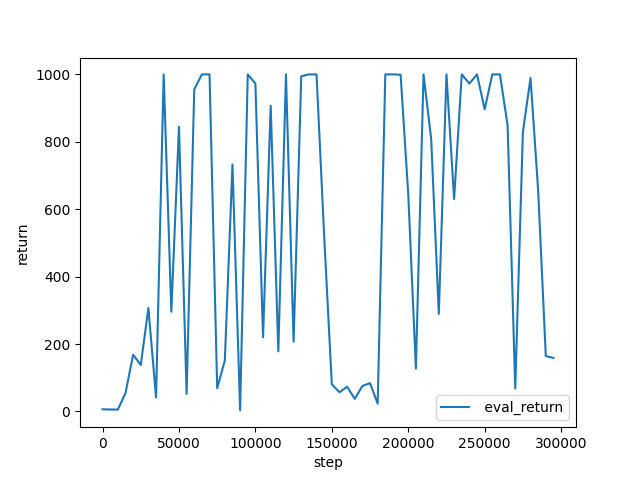
\includegraphics[width=0.6\textwidth]{../report/assets/P3-1-3-1.png}
    \caption{HalfCheetah-v4 with REINFORCE-1}
    \label{fig:halfcheetah-v4-reinforce-1}
\end{figure}

The problem is that the curve is very unstable! I can't tell the reason clearly. However, I did another experiment, which turns out to make the curve stable. The result is shown below.

\begin{figure}[H]
    \centering
    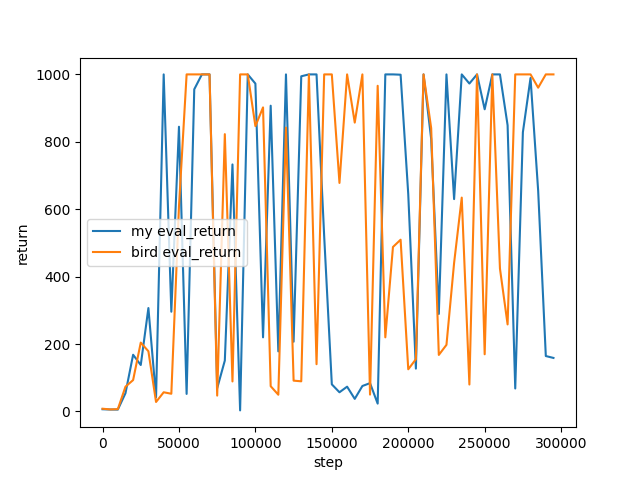
\includegraphics[width=0.45\textwidth]{../report/assets/P3-1-3-1-compare.png}
    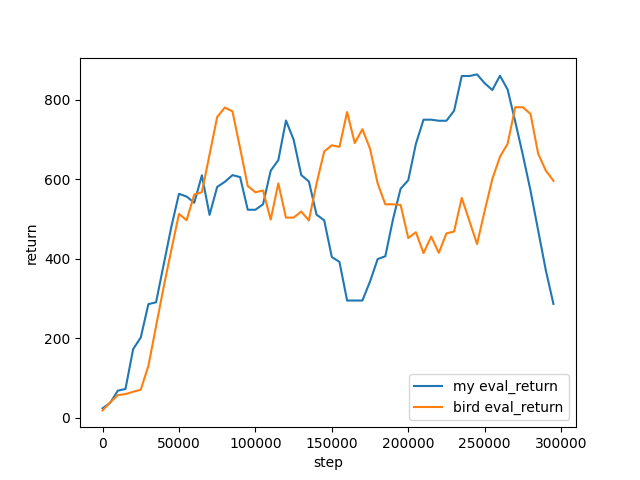
\includegraphics[width=0.45\textwidth]{../report/assets/P3-1-3-1-compare-smoothed.png}
    \caption{HalfCheetah-v4 with REINFORCE-1 (bird method); the right side is smoothed per 5 iterations}
    \label{fig:halfcheetah-v4-reinforce-1-another}
\end{figure}

The detail of the experiment is shown below: I changed the code as 
\begin{lstlisting}[language=Python]
def actor_loss_reinforce(self, obs: torch.Tensor):
    batch_size = obs.shape[0]

    action_distribution: torch.distributions.Distribution = self.actor(obs)

    with torch.no_grad():
        action = action_distribution.sample([self.num_actor_samples])
        assert action.shape == (
            self.num_actor_samples,
            batch_size,
            self.action_dim,
        ), action.shape
        if ptu.addition_args['bird method']:
            q_values = self.critic(torch.tile(obs,dims=(self.num_actor_samples,1,1)),action)
        else:
            q_values = self.target_critic(torch.tile(obs,dims= \
            
                    (self.num_actor_samples,1,1)),action)

        assert q_values.shape == (
            self.num_critic_networks,
            self.num_actor_samples,
            batch_size,
        ), q_values.shape

        q_values = torch.mean(q_values, axis=0)
        advantage = q_values

    log_probs = action_distribution.log_prob(action)
    loss = -torch.mean(log_probs*advantage)

    return loss, torch.mean(self.entropy(action_distribution))

\end{lstlisting}

In this function (also similarly in the function \verb|actor_loss_reparametrize|), If we use \verb|bird method|, then we use the \textbf{target critic} as the critic. Otherwise, we use the \textbf{critic} as the critic. 

In other words, my algorithm can be shown as

\begin{algorithm}[H]
    \caption{SAC Algorithm Implementation}
    \label{alg:sac}
    \begin{algorithmic}[1]
        \For{each step}
            \If {step $<$ some thereshold}
                \State Use random policy to collect data from the environment
            \Else
                \State Use the current policy to collect data from the environment
            \EndIf
            \State Insert the data into the replay buffer
            \If {step $<$ another thereshold}
                \State continue
            \EndIf
            \State Sample a batch of data from the replay buffer
            \State Update the critic for \textbf{num\_critic\_updates} times, using the actions from the actor
            \State Update the actor based on policy gradient or reparametrization trick with the objective being maximizing Q on \textcolor{red}{Target Critic Network}
            \State Perodically update (or momentum update) the target networks
        \EndFor
    \end{algorithmic}	
\end{algorithm}

The \verb|bird method| is almost the same, with only the red \textcolor{red}{Target Critic Network} changed to \textcolor{red}{Critic Network}. As XIBO (\url{github.com/szjzc2018}), an expert in RL, said,

\begin{quotation}
``Using the target network should be more stable.''
\end{quotation}

However, this contradicts the experiment results! So no one really know which method is really better.
    
\textbf{Deliverables}
\begin{itemize}
    \item Train an agent on \verb|HalfCheetah-v4| using the provided config (\verb|halfcheetah_reinforce1.yaml|). Note that this configuration uses only one sampled action per training example.
    \item Train another agent with \verb|halfcheetah_reinforce_10.yaml|. This configuration takes many samples from the actor for computing the REINFORCE gradient (we'll call this REINFORCE-10, and the single-sample version REINFORCE-1). Plot the results (evaluation return over time) on the same axes as the single-sample REINFORCE. Compare and explain your results.

\MYSOLUTION This figure (and the explanation) will be shown in section 3.1.4.
\end{itemize}

\subsubsection{Actor with REPARAMETRIZE}
REINFORCE works quite well with many samples, but particularly in high-dimensional action spaces, it starts to require a lot of samples to give low variance. We can improve this by using the reparametrized gradient. Parametrize $\pi_\theta$ as $\mu_\theta(s) + \sigma_\theta(s)\epsilon$, where $\epsilon$ is normally distributed. Then we can write:
\[\nabla_\theta\mathbb{E}_{s \sim \mathcal{D}, a \sim \pi_\theta(a|s)}\left[Q(s, a)\right] = \nabla_\theta\mathbb{E}_{s \sim \mathcal{D}, \epsilon \sim \mathcal{N}}\left[Q(s, \mu_\theta(s) + \sigma_\theta(s)\epsilon))\right] = \mathbb{E}_{s \sim \mathcal{D}, \epsilon \sim \mathcal{N}}\left[\nabla_\theta Q(s, \mu_\theta(s) + \sigma_\theta(s)\epsilon))\right]\]
This gradient estimator often gives a much lower variance, so it can be used with few samples (in practice, just using a single sample tends to work very well).

\textbf{Hint}: you can use \verb|.rsample()| to get a \textit{reparametrized} sample from a distribution in PyTorch.

\textbf{What you'll need to do}:
\begin{itemize}
    \item Implement \verb|actor_loss_reparametrize()|. Be careful to use the reparametrization trick for sampling!
\end{itemize}

\textbf{Testing this section}:
\begin{itemize}
    \item Make sure you can solve \verb|InvertedPendulum-v4| (use \verb|sanity_invertedpendulum_reparametrize.yaml|) and achieve similar reward to the REINFORCE case.
\end{itemize}

\MYSOLUTION The plot is shown below.

\begin{figure}[H]
    \centering
    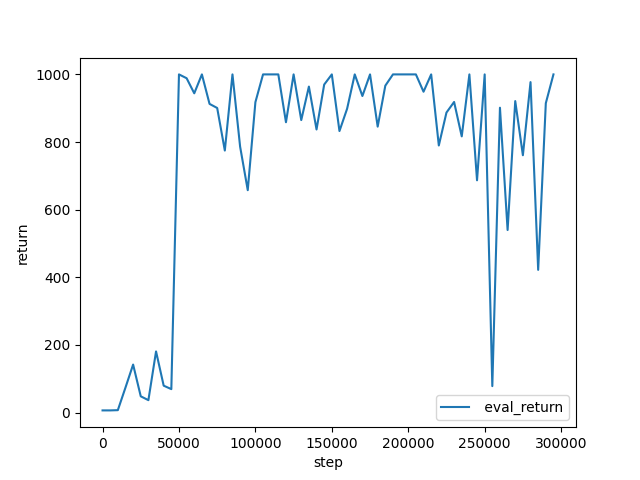
\includegraphics[width=0.6\textwidth]{../report/assets/P3-1-4-1.png}
    \caption{InvertedPendulum-v4 with REPARAMETRIZE}
    \label{fig:invert-v4-reparametrize}
\end{figure}

\textbf{Deliverables}: 
\begin{itemize}
    \item Train (once again) on \verb|HalfCheetah-v4| with \verb|halfcheetah_reparametrize.yaml|. Plot results for all three gradient estimators (REINFORCE-1, REINFORCE-10 samples, and REPARAMETRIZE) on the same set of axes, with number of environment steps on the $x$-axis and evaluation return on the $y$-axis.

\MYSOLUTION The plot is shown below.

\begin{figure}[H]
    \centering
    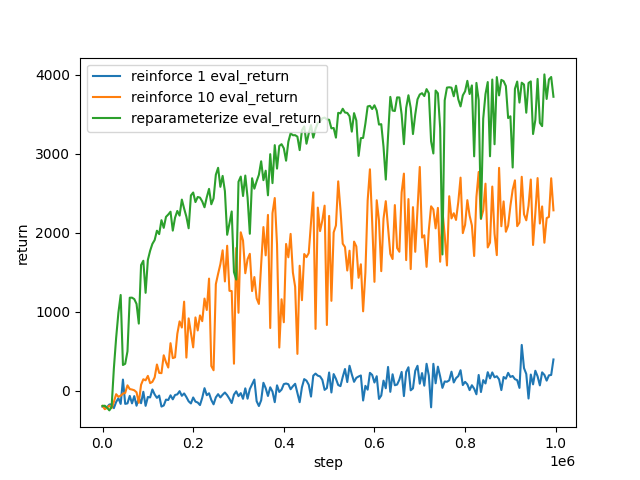
\includegraphics[width=0.6\textwidth]{../report/assets/P3-1-4-2.png}
    \caption{HalfCheetah-v4 with REPARAMETRIZE and two REINFORCE methods}
    \label{fig:halfcheetah-v4-reparametrize}
\end{figure}

For explanation (of the 3.1.3 section), the REINFORCE-10 method is better than REINFORCE-1 method, since there are more samples for REINFORCE-10 method.

    \item Train an agent for the \verb|Humanoid-v4| environment with \verb|humanoid_sac.yaml| and plot results.
    
\MYSOLUTION

This graph will be put in 3.1.5 section.

\end{itemize}

\subsubsection{Stabilizing Target Values}
As in DQN, the target $Q$ with a single critic exhibits \textit{overestimation bias}! There are a few commonly-used strategies to combat this:
\begin{itemize}
    \item Double-$Q$: learn two critics $Q_{\phi_A}, Q_{\phi_B}$, and keep two target networks $Q_{\phi_A'}, Q_{\phi_B'}$. Then, use $Q_{\phi'_A}$ to compute target values for $Q_{\phi_B}$ and vice versa:
    \[y_A = r + \gamma Q_{\phi_B'}(s', a')\]
    \[y_B = r + \gamma Q_{\phi_A'}(s', a')\]
    \item \textit{Clipped} double-$Q$: learn two critics $Q_{\phi_A}, Q_{\phi_B}$ (and keep two target networks). Then, compute the target values as $\min(Q_{\phi_A'}, Q_{\phi_B'})$.
    \[y_A = y_B = r + \gamma \min\left(Q_{\phi_A'}(s', a'), Q_{\phi_B'}(s', a')\right)\]
    \item \textbf{(Optional, bonus)} \textit{Ensembled} clipped double-$Q$: learn many critics (10 is common) and keep a target network for each. To compute target values, first run all the critics and sample two $Q$-values for each sample. Then, take the minimum (as in clipped double-$Q$). If you want to learn more about this, you can check out ``Randomized Ensembled Double-Q'': \url{https://arxiv.org/abs/2101.05982}.
\end{itemize}
Implement double-$Q$ and clipped double-$Q$ in the \verb|q_backup_strategy| function in \verb|soft_actor_critic.py|.

\textbf{Deliverables}:
\begin{itemize}
    \item Run single-$Q$, double-$Q$, and clipped double-$Q$ on \verb|Hopper-v4| using the corresponding configuration files. Which one works best? Plot the logged \verb|eval_return| from each of them as well as \verb|q_values|. Discuss how these results relate to overestimation bias.
    
\MYSOLUTION Among the four implementations, double-Q and REDQ works the best. The plot is shown below.

\begin{figure}[H]
    \centering
    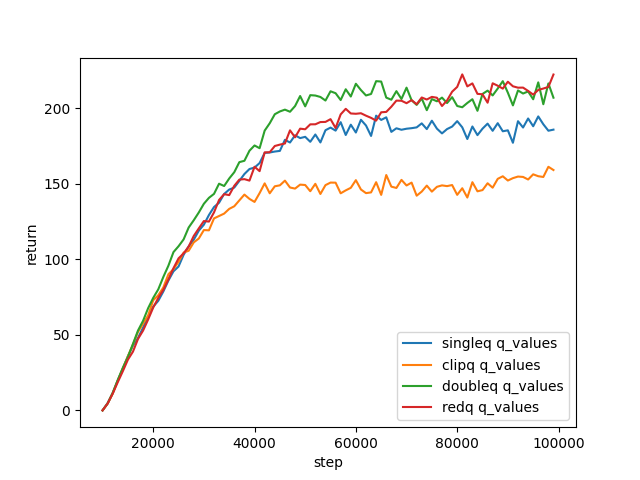
\includegraphics[width=0.4\textwidth]{../report/assets/P3-1-5-1.png}
    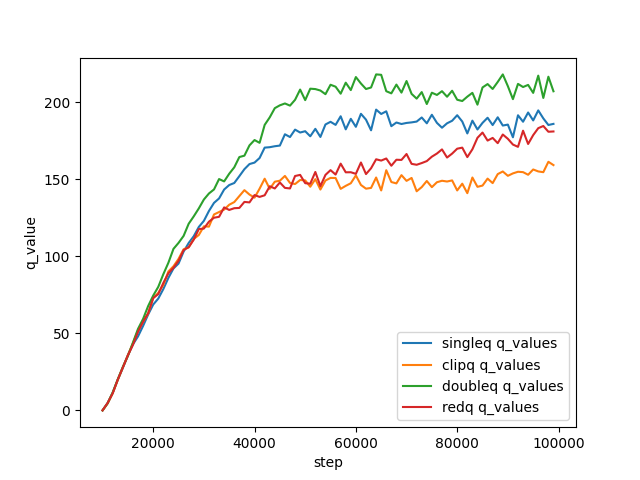
\includegraphics[width=0.4\textwidth]{../report/assets/P3-1-5-2.png}
    \caption{Hopper-v4 with single-Q, double-Q, clipped double-Q and REDQ}
    \label{fig:hopper-v4-q}
\end{figure}

From the plot of the Q values, at first glance, it seems that the double Q has largest Q values. This seems to contradict the fact that double Q reduces the Q function. However, this may due to the fact that double Q method performs best, so the Q values increase very quickly. Thus, from the Q values, we can't really tell much. On the other hand, from the performance figure, we can see that double Q indeed performs the best.

    \item Pick the best configuration (single-$Q$/double-$Q$/clipped double-$Q$, or REDQ if you implement it) and run it on \verb|Humanoid-v4| using \verb|humanoid.yaml| (edit the config to use the best option). You can truncate it after 500K environment steps. If you got results from the humanoid environment in the last homework, plot them together with environment steps on the $x$-axis and evaluation return on the $y$-axis. Otherwise, we will provide a humanoid log file that you can use for comparison. How do the off-policy and on-policy algorithms compare in terms of sample efficiency? \textit{Note: if you'd like to run training to completion (5M steps), you should get a proper, walking humanoid! You can run with videos enabled by using \texttt{-nvid 1}. If you run with videos, you can strip videos from the logs for submission with \href{https://gist.github.com/kylestach/e9964f5f34ee74367547dec83eaf5fae}{this script}.}
    
\MYSOLUTION 

\begin{figure}[H]
    \centering
    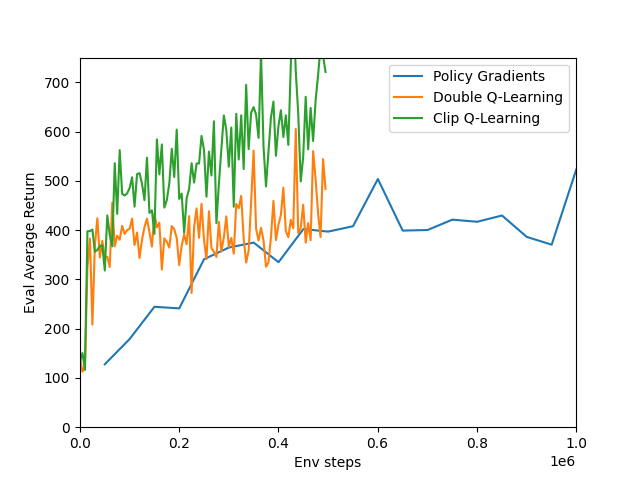
\includegraphics[width=0.6\textwidth]{../report/assets/3-1-5-3.png}
    \caption{Humanoid-v4 with double-Q}
    \label{fig:humanoid-v4-q}
\end{figure}

It is clear that off-policy methods are more sample efficient than on-policy methods. However, since the computation power is limited, I can't run the off-policy method to the end, so I can't tell which method is better in the end.
\end{itemize}

\section{Submitting the code and experiment runs}
In order to turn in your code and experiment logs, create a folder that contains the following: 
\begin{itemize}
    \item A folder named \texttt{data} with all the experiment runs from this assignment.
    % For Q-learning, you need to submit one run for Q1, two runs for Q2, and three runs for Q3. These folders can be copied directly from the \texttt{data} folder. For the actor critic section, likewise submit one folder for each run.
    \textbf{Do not change the names originally assigned to the folders, as specified by  \texttt{exp\_name} in the instructions. Video logging is disabled by default in the code, but if you turned it on for debugging, you will need to run those again with \texttt{--video\_log\_freq -1}, or else the file size will be too large for submission.}
    \item The \texttt{cs285} folder with all the \texttt{.py} files, with the same names and directory structure as the original homework repository (excluding the \texttt{data} folder). Also include any special instructions we need to run in order to produce each of your figures or tables (e.g. ``run python myassignment.py -sec2q1'' to generate the result for Section 2 Question 1) in the form of a README file.
    % Note that this assignment’s plotting must be done in a python script, such that running a single script like this can generate the plot.
\end{itemize}

As an example, the unzipped version of your submission should result in the following file structure. \textbf{Make sure that the submit.zip file is below 15MB and that they include the prefix \texttt{q1\_}, \texttt{q2\_}, \texttt{q3\_}, etc.}

\begin{forest}
  for tree={
    font=\ttfamily,
    grow'=0,
    child anchor=west,
    parent anchor=south,
    anchor=west,
    calign=first,
    edge path={
      \noexpand\path [draw, \forestoption{edge}]
      (!u.south west) +(7.5pt,0) |- node[fill,inner sep=1.25pt] {} (.child anchor)\forestoption{edge label};
    },
    before typesetting nodes={
      if n=1
        {insert before={[,phantom]}}
        {}
    },
    fit=band,
    before computing xy={l=15pt},
  }
[submit.zip
  [data
      [hw3\_dqn\_...
        [events.out.tfevents.1567529456.e3a096ac8ff4]
      ]
      [hw3\_sac\_...
        [events.out.tfevents.1567529456.e3a096ac8ff4]
        % [checkpoint]
        % [policy\_itr\_0.data-00000-of-00001]
        % [...]
      ]
      [...]
  ]
  [cs285
    [agents
        [soft\_actor\_critic.py]
        [dqn\_agent.py]
    ]
    [...]
  ]
[README.md]
    [...]
]
\end{forest}
% \todo{tree probably needs to be updated}
% \end{question}

If you are a Mac user, \textbf{do not use the default ``Compress'' option to create the zip}. It creates artifacts that the autograder does not like. You may use \texttt{zip -vr submit.zip . -x "*.DS\_Store"} from your terminal from within the top-level \verb|cs285| directory.

Turn in your assignment on Gradescope. Upload the zip file with your code and log files to \textbf{HW3 Code}, and upload the PDF of your report to \textbf{HW3}.

\newpage 

\paragraph{SAC-related questions.} 
We wanted to address some of the common questions that have been asked regarding Question 6 of the HW. The full algorithm for SAC is summarized below, the equations listed in this paper will be helpful for you: {\url{https://arxiv.org/pdf/1812.05905}}. Some definitions that will be useful:
\begin{enumerate}
    \item What is alpha and how to update it: Alpha is the entropy regularization coefficient denoting how much exploration to add to the policy. You should update based on Eq. 18 in Section 5 in the above paper as follows: 
    $$
    J(\alpha)=\mathop{\mathbb{E}}_{a_t \sim \pi_t}[-\alpha\log_{\pi_t}(a_t|s_t) - \alpha\bar{\mathcal{H}}].
    $$
    \item Target entropy is the negative of the action space dimension that is used to update the alpha term.
    \item SquashedNorm: This is a function that takes in mean and std as in previous homeworks, and will give you a distribution that you can sample your action from. 
    \item To update the critic, refer to how to update Q-function parameters in Equation 6 of the paper above as follows: \\
    $$J_{Q}(\theta) = Q_{\theta}(s_t, a_t) - (r(s_t, a_t) + \gamma (Q_{\bar{\theta}}(s_{t+1}, a_{t+1}) - \alpha \log(\pi_{\phi}(a_{t+1}, s_{t+1})))$$
    \item To update the policy, follow Equation 18: \\
    $$J(\alpha) = E_{a_t \sim \pi_t} [- \alpha \log \pi_{t}(a_t|s_t) - \alpha \bar{\mathcal{H}}]$$
    \item You don't need to alter any parameters from the SAC run commands. The correct implementation should work with the provided default parameters.
    
\end{enumerate}


\end{document}